\begin{mainquestion}{diode_conceptual}{Diode Deep Dive}
Consider a simplified physical representation of the diode assuming A
were $n$-type material and B were $p$-type material.

\begin{center}
    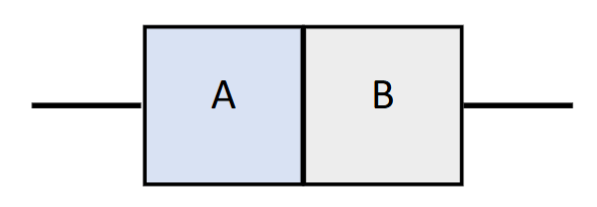
\includegraphics[width=0.6\textwidth]{questionbank/diodes/diode_conceptual/v0/diode_drawing.png}
\end{center}

% =========================================================
\begin{partquestion}{side}
{Which side is the anode? Which side is the cathode?}

\begin{answer}
The anode ($p$-side) is the terminal on side B, and the cathode ($n$-side) is the terminal on side A.
\end{answer}
\end{partquestion}

% =========================================================
\begin{partquestion}{doped}
{Which region would one dope with boron atoms? What about phosphorus atoms?}

\begin{answer}
When making a $pn$ junction, one would dope side B with boron. It will provide more free holes in the semiconductor material. Similarly, one would dope side A with phosphorus atoms to provide more free electrons in the semiconductor.
\end{answer}
\end{partquestion}

% =========================================================
\begin{partquestion}{groupiv}
{Where might one find silicon atoms? Germanium? Could you replace silicon with any
Group IV element and make a reasonable diode?}

\begin{answer}
Silicon and germanium are both Group IV elements and as such make a good base for a semiconductor. Not every Group IV element is equally suitable for constructing a practical conventional diode. Diamond, an allotrope of carbon, has a much larger bandgap than silicon or germanium and ordinarily behaves as an excellent insulator, although specialized diamond semiconductor devices can be fabricated.
\end{answer}
\end{partquestion}

% =========================================================
\begin{partquestion}{excess}
{Where are there excess holes? Where are there excess electrons?}

\begin{answer}
The excess holes are found on the $p$-type material (side B). The excess electrons are found on the $n$-type material (side A).
\end{answer}
\end{partquestion}

% =========================================================
\begin{partquestion}{charges}
{Where are the bound positive charges? Where are the bound negative charges?}

\begin{answer}
The bound positive charges are due to the phosphorus atoms in side A after they have donated their electrons. The bound negative charges are due to the boron atoms in side B after they have “donated holes” (actually they really grab electrons from the surrounding semiconductor material).
\end{answer}
\end{partquestion}

% =========================================================
\begin{partquestion}{field}
{When disconnected, does this diode generate an electric field, if so, what direction does it point? If not, what would be required to generate the field?}

\begin{answer}
Yes, this diode will have an inherent electric field due to the bound positive charges in A and the bound negative charges in B. The field therefore points from positive bound charges to negative bound charges (A to B). Note this is from the cathode to the anode!
\end{answer}
\end{partquestion}

% =========================================================
\begin{partquestion}{flow}
{When disconnected, is there current flow? Explain your answer.}

\begin{answer}
When the diode is disconnected, there is no net current flow, but there will be a diffusion current $I_D$ from B to A and a drift current $I_S$ from A to B that exactly equal one another,
that is, $I_D = I_S$. 
\end{answer}
\end{partquestion}

\end{mainquestion}